\chapter{Use Cases \\
\small{\textit{-- Author Name}}
\index{use cases} 
\index{Chapter!Use Cases}
\label{Chapter::UseCases}}

This chapter presents the use case diagrams that satisfy the requirements.
Detailed description of each use case should be given in separate chapters for each use case.
In this sample script, they are all left in this chapter.  Move them as needed.

\section{Table of Use Cases}
To prevent gold-plating all use cases must be mapped to at least one requirement.  If there are
any use cases that don't have a requirement, then the use case should be removed.  A table to 
keep track of this mapping is shown next.

\small
\begin{longtable}{|p{2cm}|p{2.5cm}|p{10.5cm}|}
\caption{Use Cases Table \label{Table::UseCases}}\\
\hline
\textbf{Use Case} & \textbf{Requirements} &\textbf{Name and Description} 
\\
\hline 
\endhead

\UseCaseReference{ucFirstUseCase} & 
\RequirementReference{reqkQuality}{reqqFirstQualityRequirement},
\RequirementReference{reqkFunctional}{reqfFirstFunctionalRequirement},
\dots
&
\UseCaseName{ucFirstUseCase} is a use case describing one of the usages of the system.
One use case may map to multiple requirements.  It must map to at least one.
\\ 
\hline

\end{longtable}

You should distill the use cases/user stories that defined in your project specification. Here you
should focus on the “must-have” use cases/stories, and elaborate each scenario to consider the
pre-conditions, post-conditions, normal flow, and exceptional flows of each use case, if this is
not considered in your project specifications.

\section{Use Case Diagrams}

\begin{figure}[h]
\centering
\psfrag{ucWHW }{\hspace{0.05in} \footnotesize \UseCaseReference{ucFirstUseCase}}
%\psfrag{ucWHW }{\hspace{0.05in} \footnotesize test}
\scalebox{1}{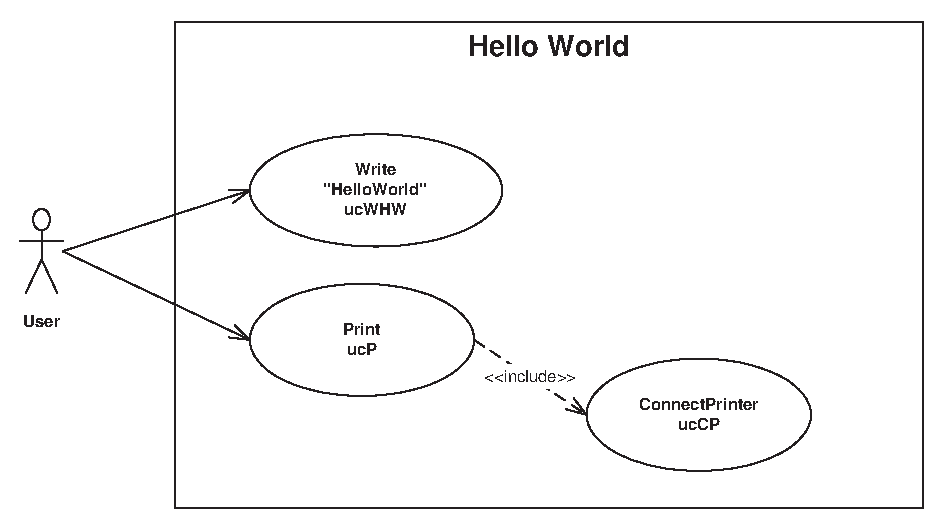
\includegraphics{eps/UseCases/dsnHelloWorld.eps}}
\caption{\FigureLabel{dsnHelloWorld}: \FigureName{dsnHelloWorld} Sample use case diagram, with 
reference to use case \UseCaseReference{ucFirstUseCase}.}
\end{figure}

\section{Use Case}
\begin{table}
\center
\caption{\TableLabel{ucFirstUseCase}. Use Case First}
\scalebox{1}{
\begin{tabular}{|p{16cm}|}
\hline
	\begin{useCase}[\UseCaseName{ucFirstUseCase}]
	\UseCaseLabel{ucFirstUseCase}
	\index{UseCase!\UseCaseName{ucFirstUseCase}}
		Write Hello World!  First use case.
	\end{useCase}  
\\
\hline
Requirements:  \RequirementReference{reqkFunctional}{reqfFirstFunctionalRequirement}
\\
\hline
Diagrams: Figure \FigureNameWIReference{dsnHelloWorld}
\\
\hline
Brief description:\\
The system writes Hello World.\\
\hline
Primary actors: \newline
User \\
\hline
Secondary actors: \\
None. \\
\hline
Preconditions:
\begin{enumerate}[topsep=0pt,itemsep=0pt,parsep=0pt,partopsep=0pt,leftmargin=12pt]
\item Item one.
\item Item two.
\end{enumerate} \\
\hline
Main flow:
\begin{enumerate}[topsep=0pt,itemsep=0pt,parsep=0pt,partopsep=0pt,leftmargin=12pt]
\item Step one.
\item Step two.
\item If this then 
	\begin{enumerate}
	[label*=\arabic*.,topsep=0pt,itemsep=0pt,parsep=0pt,partopsep=0pt,leftmargin=12pt]
	\item Step one.
	\item Step two.
	\end{enumerate}
\end{enumerate} \\
\hline
Postconditions: 
None. \\
\hline
Alternative flows:
None. \\
\hline
\end{tabular}
}
\end{table}